%&latex

\documentclass[size=12pt,display=slidesnotes]{powerdot}

\usepackage[english]{babel}
\usepackage{multicol}
\usepackage{amsmath}
\usepackage{amsthm}
\usepackage{amssymb}
\usepackage{graphicx}
\usepackage{amsfonts}
\usepackage{kbordermatrix}
\usepackage{alltt}
\usepackage{ulem}

\usepackage{listings}
\usepackage{lstpatch}

%Para poner colores en los listados xml
\usepackage[usenames,dvipsnames,svgnames,table]{xcolor}
\definecolor{Maroon}{RGB}{255,100,0}


%Definir las caracteristicas de los listados
\lstdefinelanguage{XML}
{
  basicstyle=\ttfamily\scriptsize,
  morestring=[b]",
  moredelim=[s][\bfseries\color{black}]{<}{\ },
  moredelim=[s][\bfseries\color{black}]{</}{>},
  moredelim=[l][\bfseries\color{Maroon}]{/>},
  moredelim=[l][\bfseries\color{Maroon}]{>},
  morecomment=[s]{<?}{?>},
  morecomment=[s]{<!--}{-->},
  commentstyle=\color{DarkOliveGreen},
  stringstyle=\color{blue},
  identifierstyle=\color{red},
}
\lstset{language=XML,
        columns=flexible,
        breaklines=true
        }

%Para usar m�ltiples columnas
\usepackage{multicol} 
\setlength{\columnsep}{5pt}

%para lineas intermitentes
\usepackage{arydshln}

\begin{document}

%+Title
\title{SECURITY IN PETRI NETS SHARING AND STORAGE: SUBNETS, PRIVACY, INTEGRITY,
AUTHENTICATION AND NON REPUDIATION}


\author{\textbf{I\~nigo Le\'on Samaniego}
\\
\\\textbf{Defensa de Tesis Doctoral}\\
Universidad de La Rioja
\\
\\
\begin{small}Directores: Emilio Jim\'enez Mac\'ias,
Juan Ignacio Latorre Biel\end{small}
\\
}

\maketitle
%-Title




\section{Introducci\'on}
\begin{slide}{Marco}
\begin{Large}Las Redes de Petri...\end{Large}
\pause\bigskip
\begin{itemize}
\item ...est\'an muy extendidas para modelar sistemas
      \begin{itemize}\begin{small}
      \item servicios y procesos log\'isticos
      \item sistemas concurrentes
      \item ...
      \end{itemize}\end{small}
      \pause\bigskip
\item ...est\'an descritas de una manera exhaustiva, con informaci\'on de toda la red
\pause\bigskip
\item ...pueden ser modificadas sin control de integridad o autor\'ia
\end{itemize}
\end{slide}






\begin{slide}{Problema}
\begin{Large}Pero es posible que...\end{Large}
\pause\bigskip
\begin{itemize}
\item ...no queramos describir la red entera
\pause\bigskip
\item ...parte del proceso sea secreto para personas no autorizadas
\pause\bigskip
\item ...necesitemos validaci\'on de partes concretas por parte de determinadas
personas
\pause\bigskip
\item ...queramos evitar cualquier modificaci\'on
no autorizada
\end{itemize}
\end{slide}




\begin{slide}{Justificaci\'on de la investigaci\'on}
Ser\'ia interesante proveer de seguridad a las redes de Petri...
\pause\bigskip
\begin{itemize}
\item ...ocultando partes concretas
\pause\bigskip
\item ...detectando modificaciones  no autorizadas
\pause\bigskip
\item ...autentic\'andola (o una parte de ella)
\pause\bigskip
\item ...evitando suplantaci\'on de identidades
\end{itemize}
\end{slide}



\begin{slide}{Contribuciones}
Mis \begin{large}\textbf{contribuciones originales}\end{large} al conocimiento son:
\pause\bigskip
\begin{enumerate}
\item Estudio en profundidad de subredes, abstrayendo su estructura interna
del exterior a trav\'es de interfaces
\pause\bigskip
\item M\'etodo para construir estas subredes e interfaces a partir de la representaci\'on matricial
\pause\bigskip
\item Descripci\'on de una posible extensi\'on de PNML para la representaci\'on
de subredes
\pause\bigskip
\item Aplicaci\'on de t\'ecnicas de seguridad a las redes representadas de
esta manera
\end{enumerate}
\end{slide}



\section{Subredes}
\begin{slide}{Conceptos y Definiciones}

\begin{itemize}
 \item Sea $R=\langle P,T,\alpha,\beta\rangle$
una red de Petri. Una subred de $R$ es otra red $\overline {R}=\langle\overline{P},\overline{T},\overline{\alpha},\overline{\beta}\rangle$
tal que  $\overline{P}\subseteq P$ y $\overline{T}\subseteq T$, $\overline{\alpha}$
y $\overline{\beta}$ son restricciones de \alpha$ y $\beta$ sobre
$\overline{P}\times\overline{T}$.
\pause
\bigskip
\item Usando matrices:
\begin{footnotesize}
{\setlength{\arraycolsep}{1pt}
\[
C=
\kbordermatrix{
   &t_1&t_2&t_3&t_4&t_5&t_6\\
p_1&-1 & 0 & 1 & 0 & 0 & 0\\
p_2&-1 & 0 & 0 & 1 & 0 & 0\\
p_3&1 & 0 & 0 & 0 & 0 & 0\\
p_4&0 & -1 & -1 & 0 & 0 & 0\\
p_5&0 & 1 & 0 & -1 & -1 & 1\\
p_6&0 & 0 & 0 & 0 & 1 & -1\\
}
\xrightarrow[t_1,t_2,t_3]{p_1,p_3,p_4,p_5}
C'=
\kbordermatrix{
   &t_1&t_2&t_3\\
p_1&-1 & 0 & 1 \\
p_3&1 & 0 & 0 \\
p_4&0 & -1 & -1 \\
p_5&0 & 1 & 0 \\
}
\]
}%fin de arraycolsep
\end{scriptsize}
\pause
\item $Q=\{R_1, R_2, ... R_k\}$ es una partici\'on de $R$ si
  \begin{itemize}
   \item $R_1 \cup R_2 \cup ... \cup R_k = R$
   \item $\forall i, j | 1\leqslant i, j \leqslant k, i \neq j\ \Rightarrow\ R_i \cap R_j = \emptyset$
  \end{itemize}
\end{itemize}
\end{slide}




\begin{slide}[toc=Descomposici\'on]{Descomposici\'on en subredes}
Los lugares de $\overline P$ y las transiciones de $\overline T$ pueden ser
reordenadas poni\'endolas al principio de la matriz de incidencia\footnote{Se
prueba que es una relaci\'on de equivalencia}...
{\setlength{\arraycolsep}{2pt}
\[
C=
\kbordermatrix{
& t_{1} & \cdots & t_{s} &  & t_{s+1} &  \cdots &  t_{m}\\
p_1 & a_{11} & \cdots & a_{1s} &\omit\vline & a_{1(s+1)} & \cdots & a_{1m}\\
\vdots & \vdots & \ddots & \vdots & \omit\vline & \vdots & \ddots & \vdots\\
p_r & a_{r1} & \cdots & a_{rs} & \omit\vline& a_{r(s+1)} & \cdots & a_{rm}\\
\cline{2-8}
p_{r+1} &a_{(r+1)1} & \cdots & a_{(r+1)s} & \omit\vline& a_{(r+1)(s+1)} & \cdots & a_{(r+1)m}\\
\vdots & \vdots & \ddots & \vdots & \omit\vline& \vdots & \ddots & \vdots\\
p_n & a_{n1} & \cdots & a_{ns} & \omit\vline& a_{n(s+1)} & \cdots & a_{nr}
}
\]
}%fin de arraycolsep
dividi\'endola en 4 partes:
\end{slide}



\begin{slide}[toc=Descomposici\'on II]{Descomposici\'on en subredes}
\bigskip
\[
C=
\left(\begin{array}{cc}
 N_{1} & PIM_{12}\\
 TIM_{12} & N_{2}
\end{array}\right)
\]

\begin{itemize}
\item $N_{1}$ es la subred formada por los lugares y las transiciones que
queremos agrupar en una subred
\item $N_{2}$ es la subred complementaria de $N_{1}$ y formada por el resto de lugares
y transiciones
\item $PIM_{12}$ (Places Influence Matrix) define la interacci\'on entre lugares
de $N_1$ y transiciones de $N_2$
\item $TIM_{12}$ (Transitions Influence Matrix) define la interacci\'on de
las transiciones de $N_1$ y los lugares de $N_2$\end{itemize}
$PIM_{12}$ y $TIM_{12}$ se utilizar\'an para crear el front-end de $N_1$
\end{slide}




\begin{slide}[toc=Descomposici\'on III]{Descomposici\'on en subredes}
\begin{multicols}{2}
\[
 \begin{array}{c}
  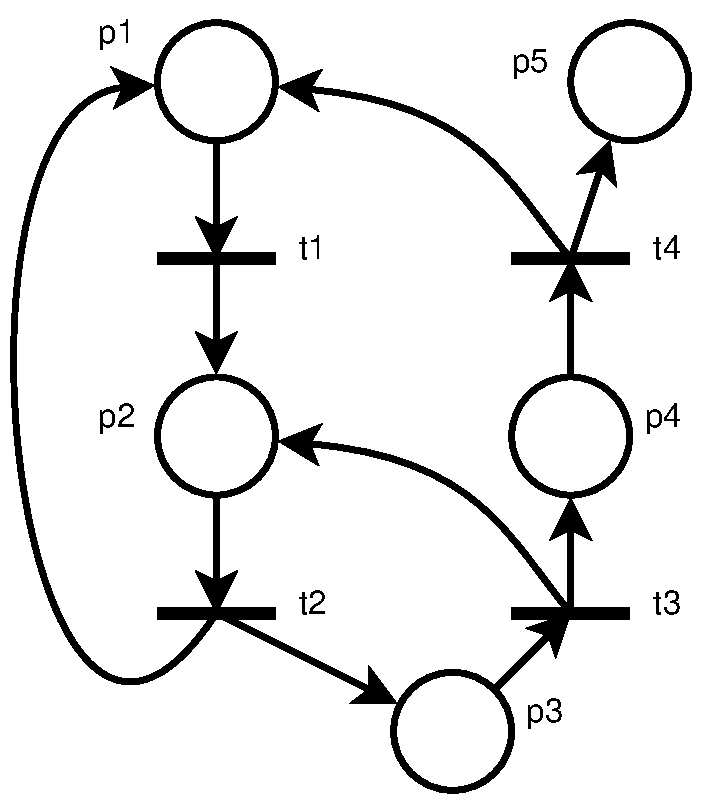
\includegraphics[width=0.25\textwidth]{figures/EleccionSubredZonasInfluencia_1.eps}\\
 
  \Downarrow \\
  
  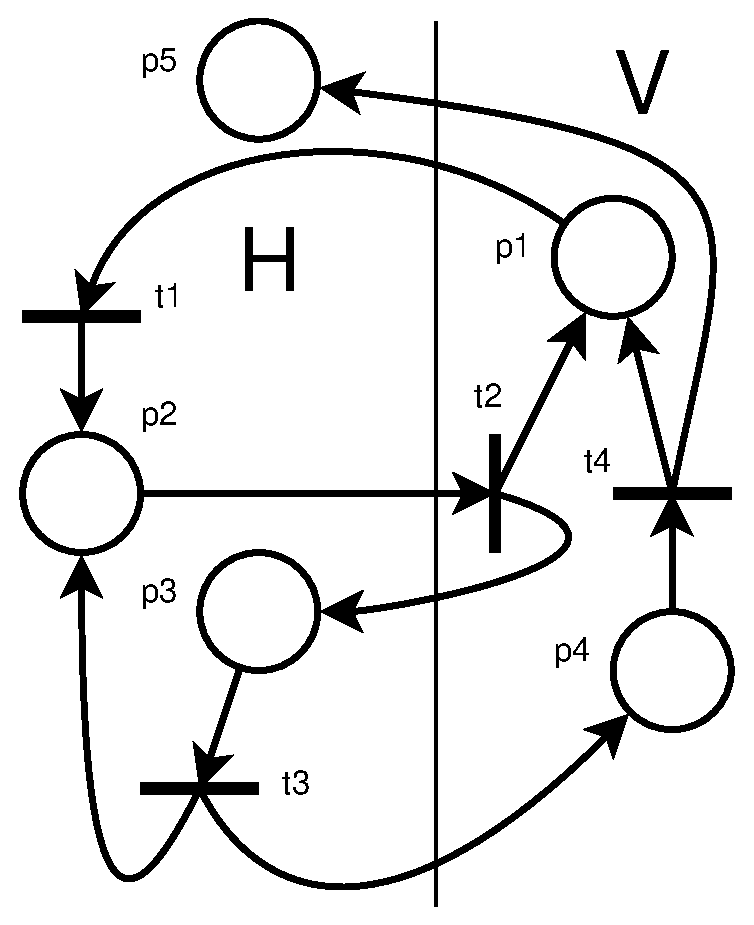
\includegraphics[width=0.25\textwidth]{figures/EleccionSubredZonasInfluencia_3.eps}
\end{array}
\]
\columnbreak
\[
\begin{array}{c}
\kbordermatrix{
   & t_1 & t_2 & t_3 & t_4\\
p_1& -1 &  1  &  0  &  1 \\
p_2&  1 & -1  &  1  &  0 \\
p_3&  0 &  1  & -1  &  0 \\
p_4&  0 &  0  &  1  & -1 \\
p_5&  0 &  0  &  0  &  1 \\
}\\
\ \\
\ \ \ \ \Downarrow\\

\kbordermatrix{
   & t_1& t_3 & \vline &t_2 & t_4\\
p_2&  1 &  1  & \vline & -1  &  0 \\
p_3&  0 & -1  & \vline &  1  &  0 \\
p_5&  0 &  0  & \vline &  0  &  1 \\
\hline
p_1& -1 &  0  & \vline &  1  &  1 \\
p_4&  0 &  1  & \vline &  0  & -1 \\
}
\end{array}
\]
\end{multicols}
\end{slide}







\begin{slide}[toc=Descomposici\'on IV]{Descomposici\'on en subredes}
\[
 \begin{matrix} 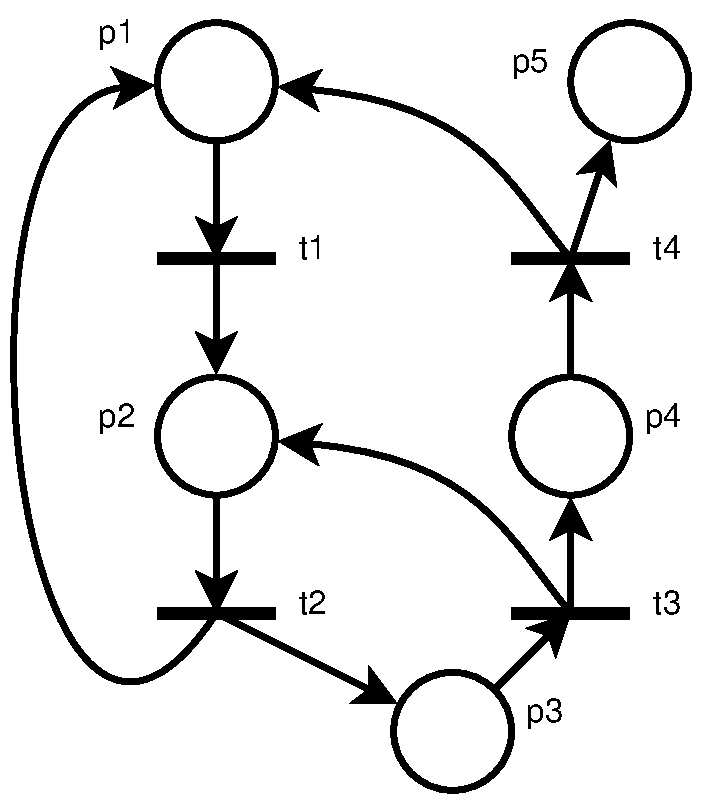
\includegraphics[width=0.3\textwidth]{figures/EleccionSubredZonasInfluencia_1.eps}\end{matrix}
  \ \ \ \ \ \ \ \ \pause
 \begin{matrix}  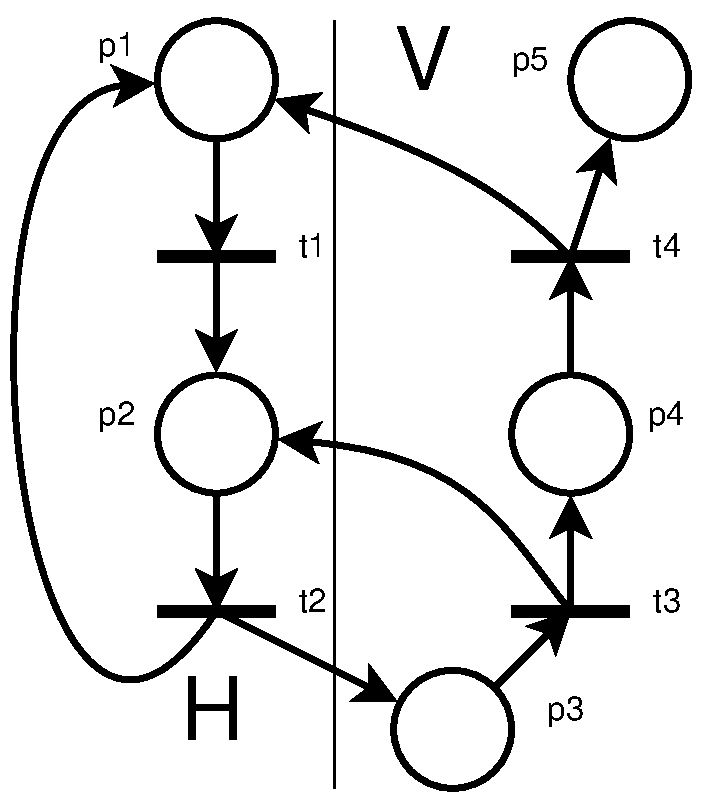
\includegraphics[width=0.3\textwidth]{figures/EleccionSubredZonasInfluencia_2.eps}\end{matrix}
\]
\[
  \ \ \pause
 \begin{matrix} 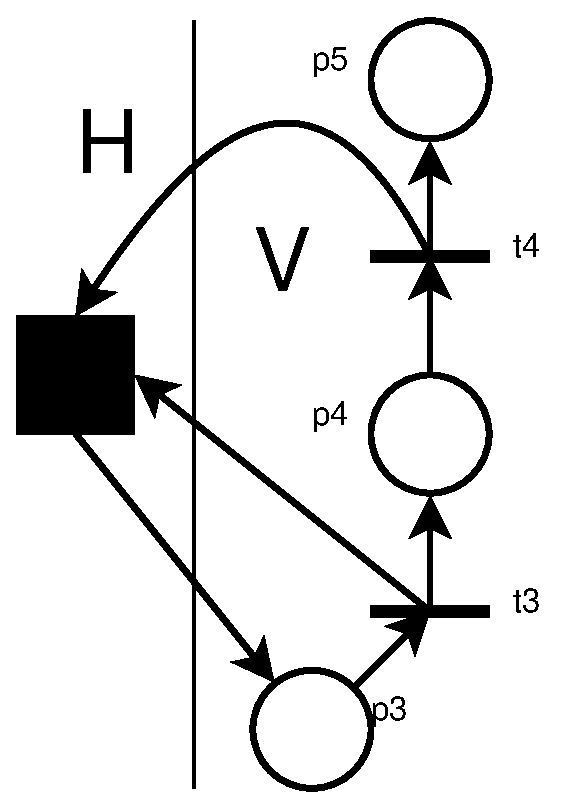
\includegraphics[width=0.235\textwidth]{figures/OcultacionSubred_1.eps}\end{matrix}
  \ \ \ \ \ \ \ \ \pause
 \mbox{?`C\'omo representar esto?}
\]
\end{slide}










\begin{slide}{Front-end}
Sea la siguiente red de Petri y su matriz de incidencia
\begin{small}
{\setlength{\arraycolsep}{2pt}
\[
\begin{matrix} 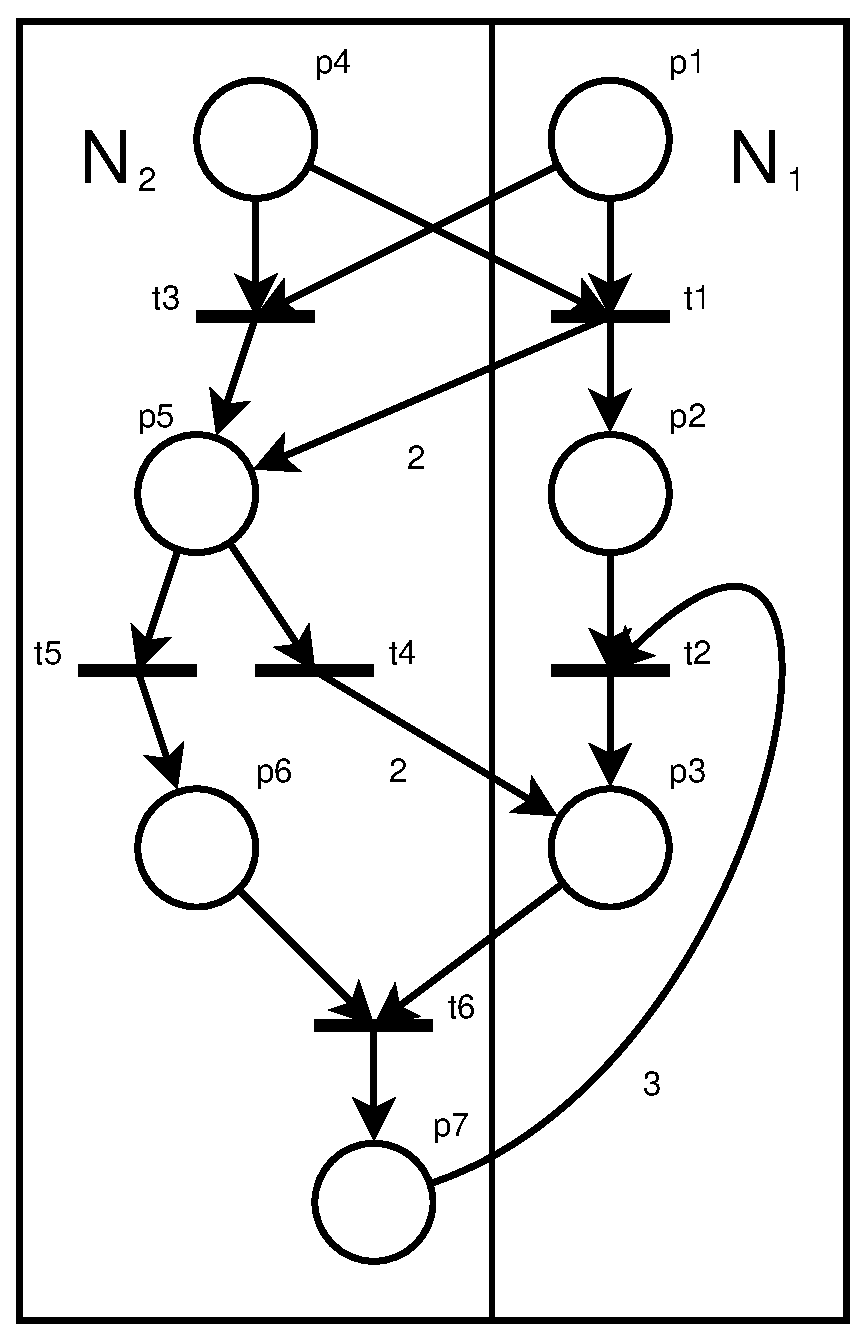
\includegraphics[width=0.35\textwidth]{figures/NodosEntradaSalidaV.eps}\end{matrix}
\ \ \ \ \
C=
\kbordermatrix{
   & t_1 & t_2 & \vline & t_3 & t_4 & t_5 & t_6\\
p_1& -1 &  0  &  \vline & -1  &  0 & 0  &  0 \\
p_2&  1 & -1  &  \vline & 0  &  0 & 0  &  0 \\
p_3&  0 &  1  &  \vline & 0 &  2 & 0  &  -1 \\
\hline
p_4&  -1 &  0  &  \vline & -1  & 0 & 0  &  0 \\
p_5&  2 &  0  &  \vline & 1  &  -1 & -1  &  0 \\
p_6&  0 &  0  &  \vline & 0  &  0 & 1  &  -1 \\
p_7&  0 &  -3  &  \vline & 0  &  0 & 0  &  1 \\
}
\]
}%fin setlength
\end{small}
\end{slide}





\begin{slide}[toc=Front-end II]{Front-end}
\begin{itemize}
  \item $\left\{ \begin{array}{l}
                \mbox{Input}\\
                \mbox{Output}
                \end{array}\right\}
        $
        gate
        $\left\{ \begin{array}{l}
                \mbox{Place}\\
                \mbox{Transition}
                \end{array}\right\}
        $
        \begin{footnotesize}(igp, igt, ogp, ogt)\end{footnotesize}
        
\[
 \begin{matrix} 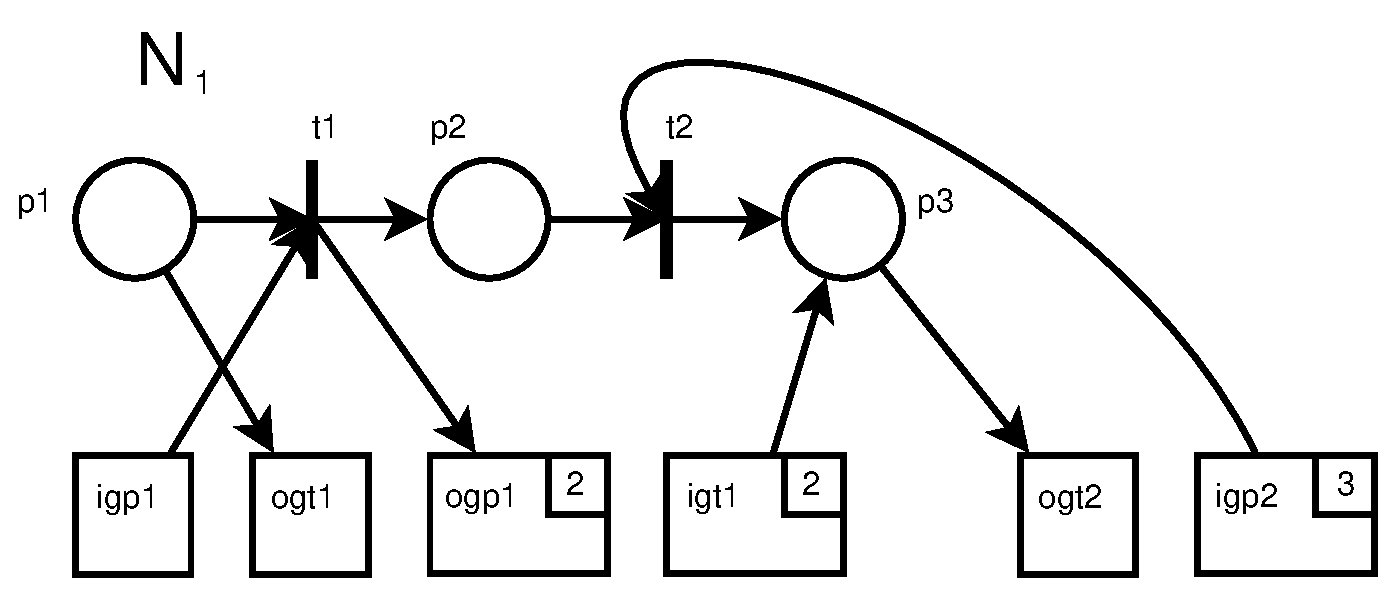
\includegraphics[width=0.5\textwidth]{figures/PuertasEntradaSalida_1.eps}\end{matrix}
\]
        \\

        \pause
\[
 \begin{matrix} 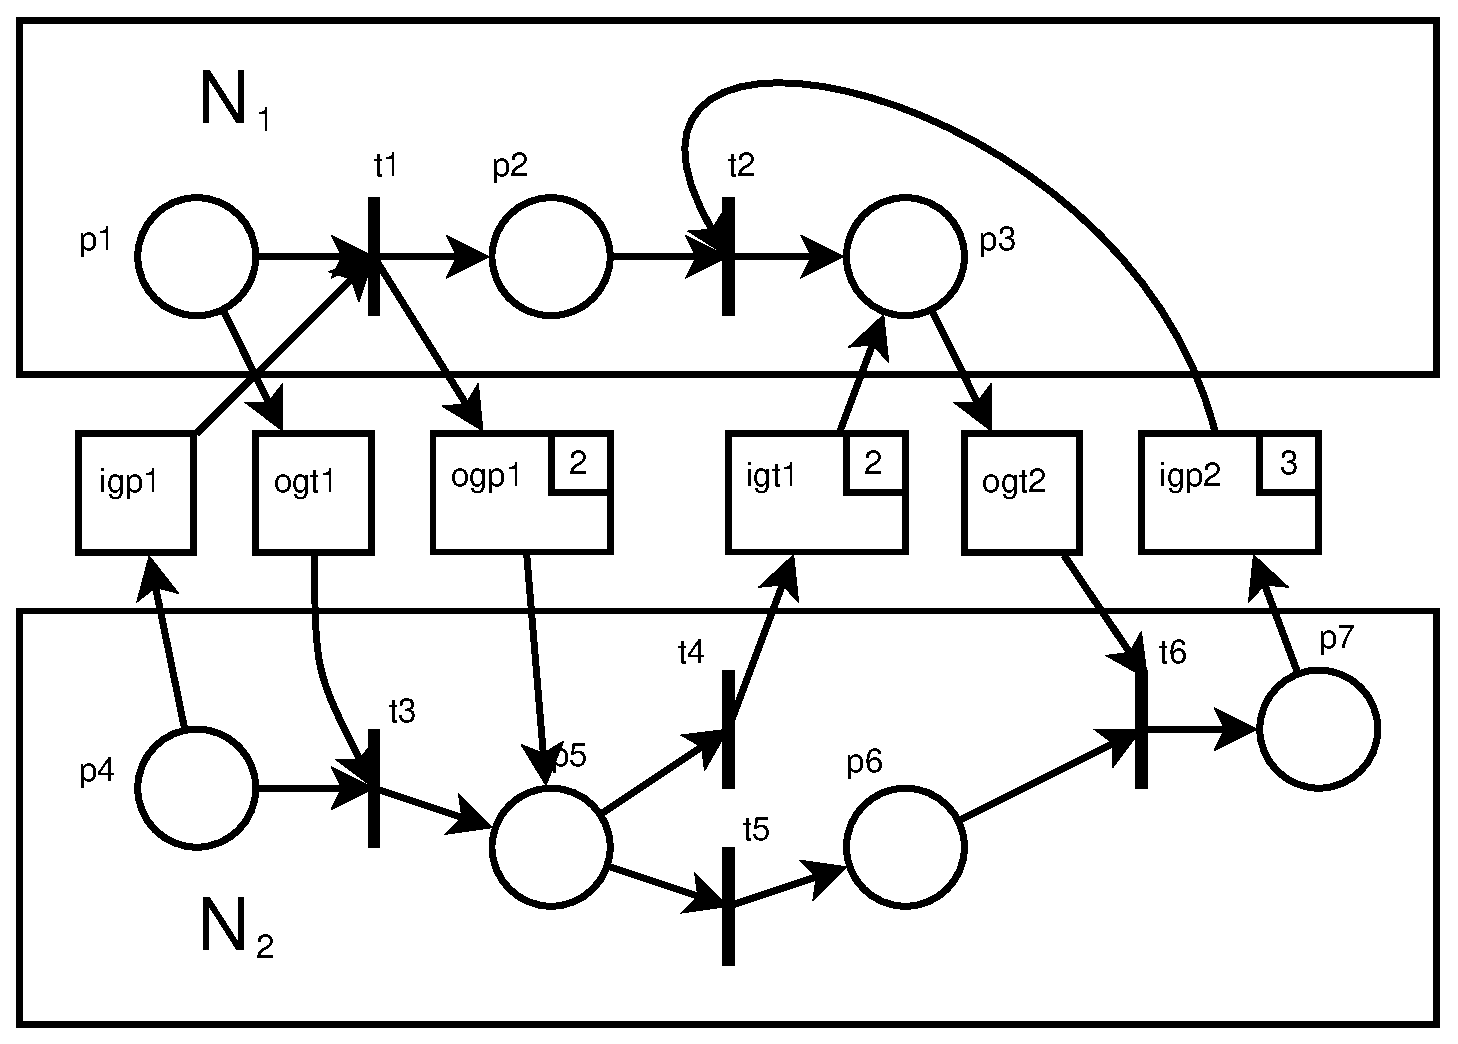
\includegraphics[width=0.5\textwidth]{figures/PuertasEntradaSalida_2.eps}\end{matrix}
\]
\end{itemize}
\end{slide}




\begin{slide}[toc=Front-end III]{Front-end}
\begin{itemize}
  \item $\left\{ \begin{array}{l}
                \mbox{Input}\\
                \mbox{Output}
                \end{array}\right\}
        $ front-end 
        $ \begin{footnotesize}\end{footnotesize}$
        \bigskip
\end{itemize}
\[
 \begin{matrix} 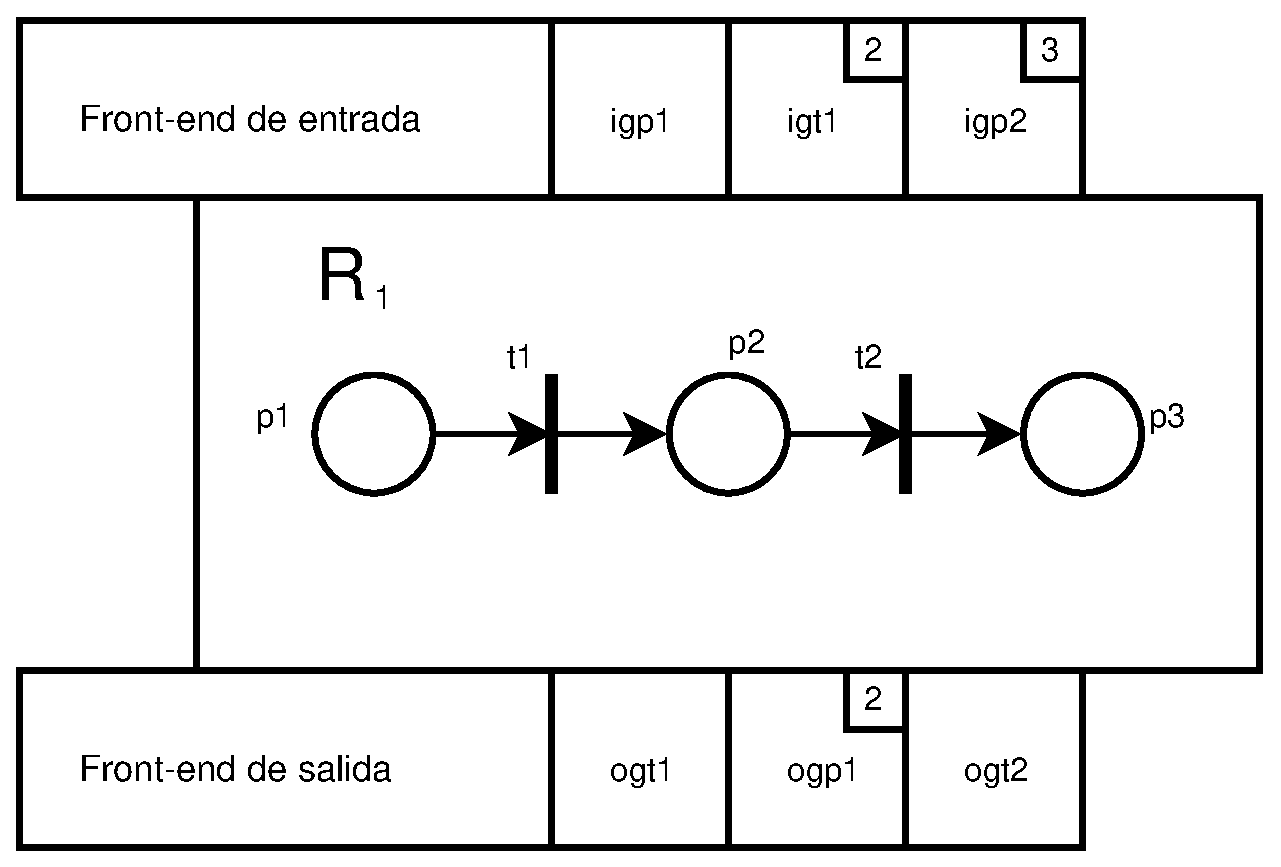
\includegraphics[width=0.63\textwidth]{figures/Front-end.eps}\end{matrix}
\]
\end{slide}




\begin{slide}[toc=Front-end IV]{Front-end}
Retomando la matriz de la red de Petri
del ejemplo
\begin{scriptsize}
{\setlength{\arraycolsep}{2pt}
\[
PIM_{12}=
\kbordermatrix{
   & t_3 & t_4 & t_5 & t_6\\
p_1&-1  &  0 & 0  &  0 \\
p_2& 0  &  0 & 0  &  0 \\
p_3& 0 &  2 & 0  &  -1 \\
}
\ \ \ \ 
TIM_{12}=
\kbordermatrix{
   & t_1 & t_2 \\
p_4&  -1 &  0  \\
p_5&  2 &  0  \\
p_6&  0 &  0  \\
p_7&  0 &  -3  \\
}
\]
}%fin setlength
\end{scriptsize}

De $PIM_{12}$ obtenemos $\left\{ \begin{array}{l}
                \mbox{igt por cada elemento \textgreater\ 0}\\
                \mbox{ogt por cada elemento \textless\ 0}
                \end{array}$

\bigskip

De $TIM_{12}$ obtenemos $\left\{ \begin{array}{l}
                \mbox{igp por cada elemento \textless\ 0}\\
                \mbox{ogp por cada elemento \textgreater\ 0}
                \end{array}$

\bigskip

As\'i, de la representaci\'on matricial podemos sacar el front-end sin necesidad
de dibujar nada
\end{slide}





\begin{slide}{Red acoplable}
Una red acoplable es una cu\'adrupla $R_a=\langle R,F,f_i,f_o\rangle$.
\pause
\begin{itemize}
 \item Parte p\'ublica: $F$
 \item Parte privada: $R$, $f_i$ y $f_o$, siendo
    \begin{itemize}
    \item $f_i: IG \to R_{i}$ la funci\'on de entrada
    \item $f_o: R_{i} \to OG$ la funci\'on de salida
    \end{itemize}
\end{itemize}
\pause
\[
 \begin{matrix} 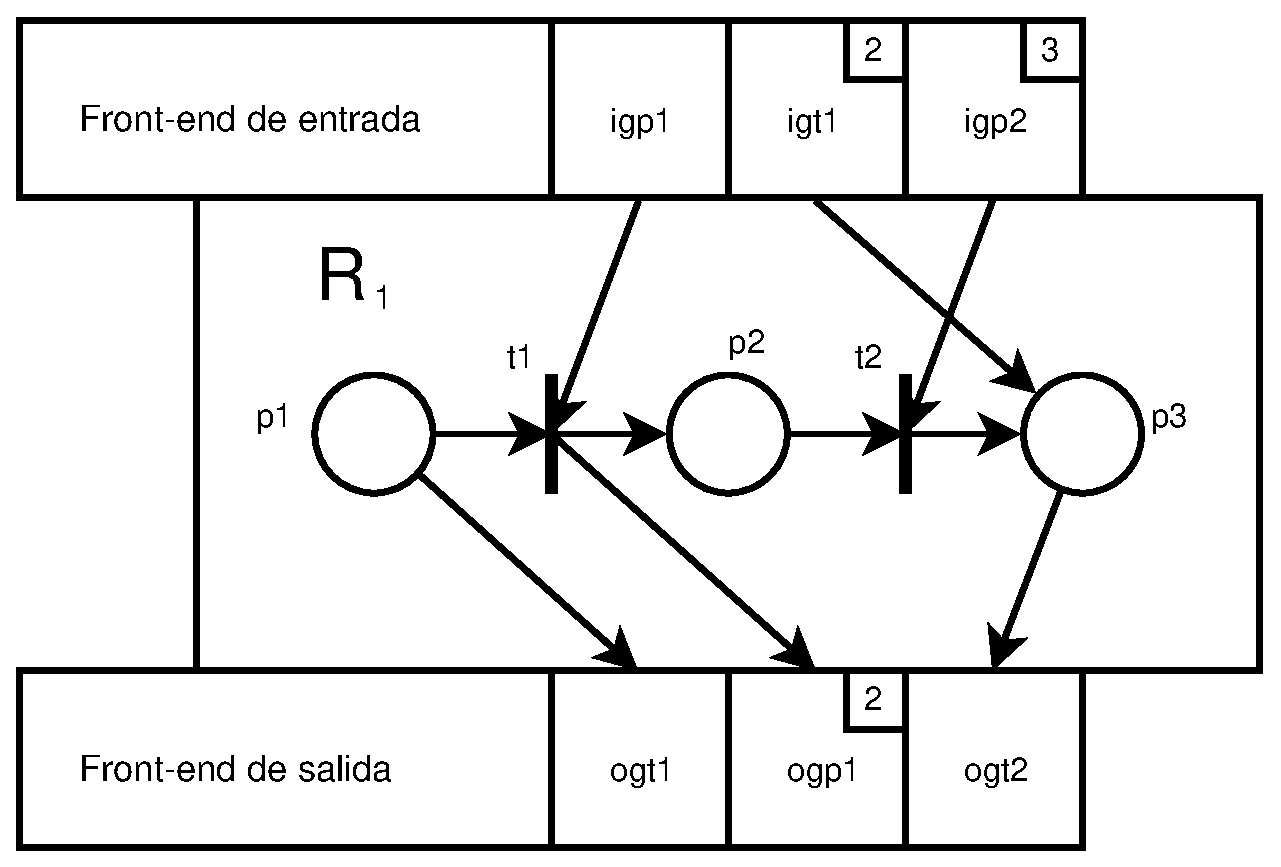
\includegraphics[width=0.63\textwidth]{figures/RedAcoplable_1.eps}\end{matrix}
\]
\end{slide}




\begin{slide}[toc=Red acoplable II]{Red acoplable}
\[
 \begin{matrix} 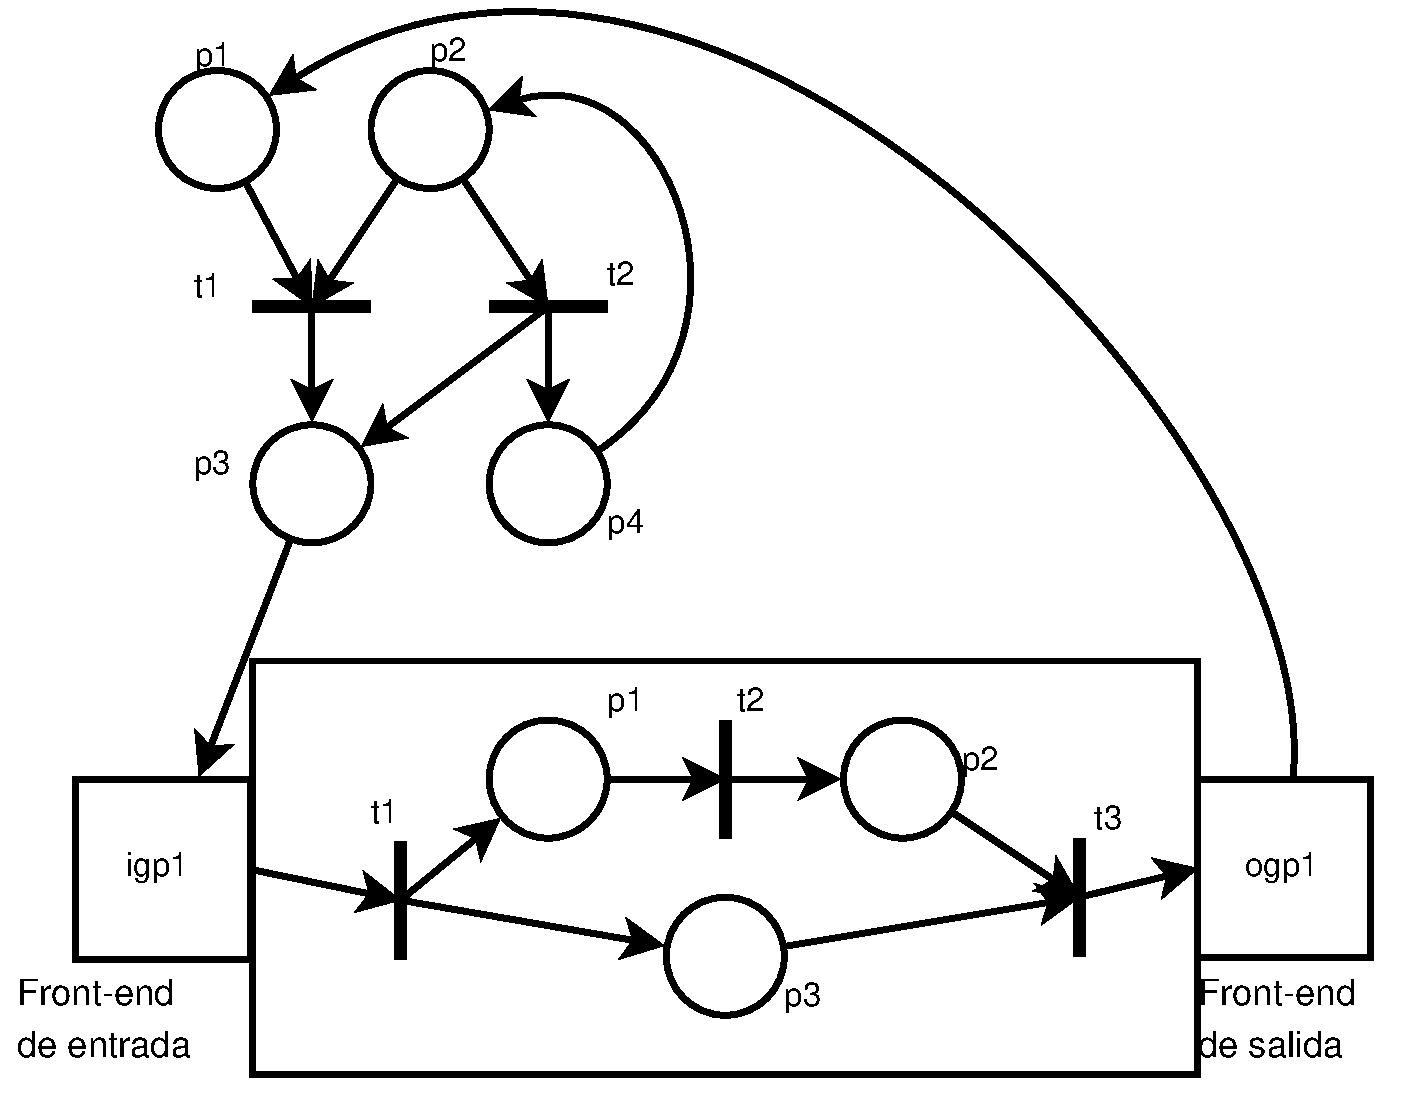
\includegraphics[width=0.45\textwidth]{figures/RedAcoplableProveedor_1.eps}\end{matrix}
\]
\pause
\[
 \begin{matrix}  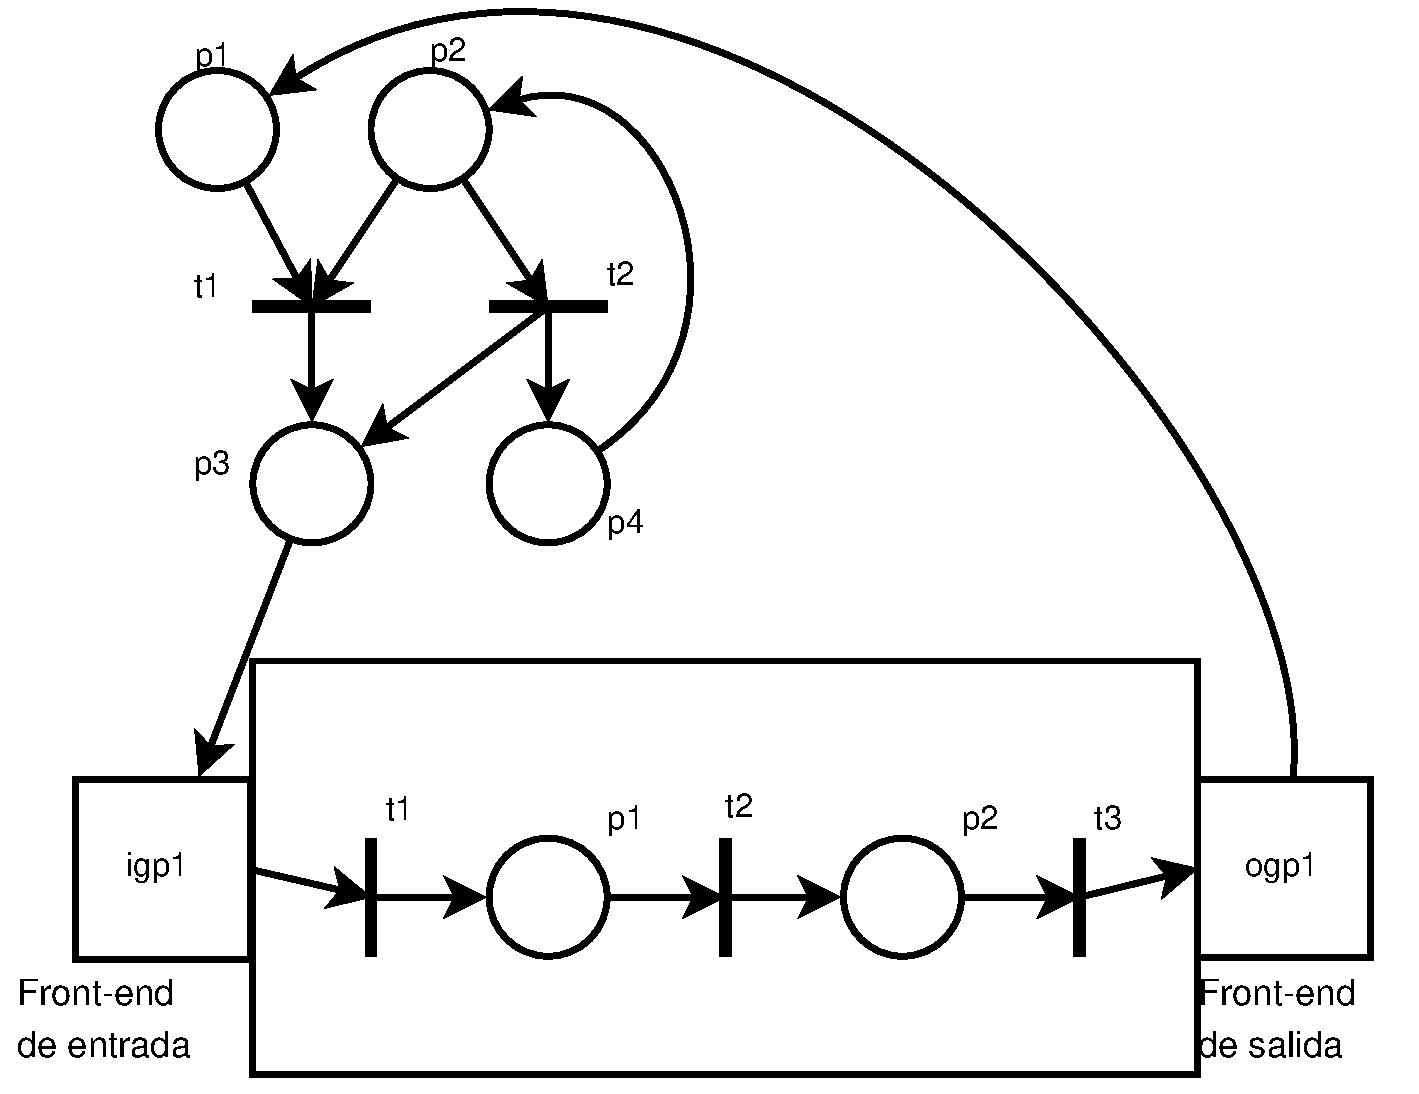
\includegraphics[width=0.45\textwidth]{figures/RedAcoplableProveedor_2.eps}\end{matrix}
\]
\end{slide}





\section{PNML}
\begin{slide}[toc=Revisi\'on PNML]{Revisi\'on general de PNML}
Objetivo:
\begin{enumerate}
\item Representar subredes de una red de Petri
\item Incluir interfaces de entrada y salida para cada subred
\end{enumerate}
\pause
\bigskip
Usarremos PNML, pero:
\begin{itemize}
\item Es un lenguaje XML para representar redes de Petri
\item No tiene capacidad para representar subredes
\end{itemize}
\pause
\bigskip
Por tanto necesitamos modificar/ampliar la gram\'atica de PNML para conseguir
los objetivos
\end{slide}



\begin{slide}[method=file,toc=Revisi\'on PNML II]{Revisi\'on general de PNML}
PNML est\'a basado en XML. Por tanto:
\begin{enumerate}
\item Comienza con una l\'inea con informaci\'on del fichero
  \begin{lstlisting}
  <?xml version="1.0" encoding="utf-8"?>
  \end{lstlisting}
\item Cada elemento tiene un id \'unico dentro del fichero
\item La estructura general es la siguiente:
\begin{lstlisting}
<?xml version="1.0" encoding="utf-8"?>
<pnml>
  <net id="myNet" type="http://www.pnml.org/version-2009/grammar/ptnet">
    <name>
      <text> My new net </text>
    </name>
    <page id="page1">
      .......
    </page>
  </net>
</pnml>
\end{lstlisting}
\end{enumerate}
\end{slide}



\begin{slide}[method=file,toc=Revisi\'on PNML III]{Revisi\'on general de PNML}
Los principales elementos son:
\begin{multicols}{2}
\begin{itemize}
\item Lugar: con un id
\begin{lstlisting}
<place id="p1">
  <name>
    <text>Lugar 1</text>
  </name>
  <initialMarking>
    <text> 2 </text>
  </initialMarking>
</place>
\end{lstlisting}
\pause
\item Transicion: con otro id
\begin{lstlisting}
<transition id="t2">
  <name>
   <text>Transicion 2</text>
  </name>
</transition>
\end{lstlisting}
\pause
\item Arco: con un id, un origen y un destino
\begin{lstlisting}
<arc id="a1" source="p1" target="t2">
  <name>
    <text>Arco 1</text>
  </name>
  <inscription>
    3
  </inscription>
</arc>
\end{lstlisting}
\bigskip
\end{itemize}
\end{multicols}
 
\end{slide}





\begin{slide}[method=file,toc=Revisi\'on PNML IV]{Revisi\'on general de PNML}
Por claridad, obviaremos algunas etiquetas.
\begin{itemize}
\item Lugar
\begin{lstlisting}
<place id="p1">
  <initialMarking>
    <text> 2 </text>
  </initialMarking>
</place>
\end{lstlisting}
\item Transicion
\begin{lstlisting}
<transition id="t2"/>
\end{lstlisting}
\item Arco
\begin{lstlisting}
<arc id="a1" source="p1" target="t2">
  <inscription> 3 </inscription>
</arc>
\end{lstlisting}
\bigskip
\end{itemize}

\end{slide}






\begin{slide}[toc=Extensi\'on PNML, method=file]{Elementos extendidos PNML:
Subnet}
Elementos extendidos en PNML:
\begin{itemize}
\item Subnet
\begin{lstlisting}[basicstyle=\ttfamily\small]
<subnet id="sn1">
  <interface id="sn1-interface">
    ...
  </interface>
  <content id="sn1-content">
    ...
  </content>
</subnet>
\end{lstlisting}
\end{itemize}
\end{slide}




\begin{slide}[toc=Extensi\'on PNML II, method=file]{Elementos extendidos PNML: Interface}
\begin{itemize}
\item Interface
\begin{lstlisting}[basicstyle=\ttfamily\small]
<interface id="sn1-interface">
  <gate id="igp1" action="input" type="place"/>
  <gate id="igp2" action="input" type="place"/>
  <gate id="ogt1" action="output" 
         type="transition">
    <inscription>
      <text> 2 </text>
    </inscription>
  </gate>
</interface>
\end{lstlisting}
\end{itemize}
\end{slide}





\begin{slide}[toc=Extensi\'on PNML III, method=file]{Elementos extendidos PNML: Content}
\begin{itemize}
\item Content
\begin{lstlisting}[basicstyle=\ttfamily\small]
  <content id="sn1-content">
    <place id="p2"/>
    <place id="p3"/>
    <transition id="t3"/>
    <arc id="sn1-a2" source="igp2" target="p2"/>
    <arc id="sn1-a3" source="igp1" target="p3"/>
    <arc id="sn1-a4" source="p3" target="ogt1">
      <inscription>
        <text> 2 </text>
      </inscription>
    </arc>
    <arc id="a5" source="t3" target="p3"/>
    <arc id="a6" source="p2" target="t3"/>
  </content>
\end{lstlisting}
\end{itemize}
\end{slide}






\begin{slide}[toc=Extensi\'on PNML IV]{Ejemplo extensi\'on PNML}
Ejemplo:
\[
\begin{matrix} 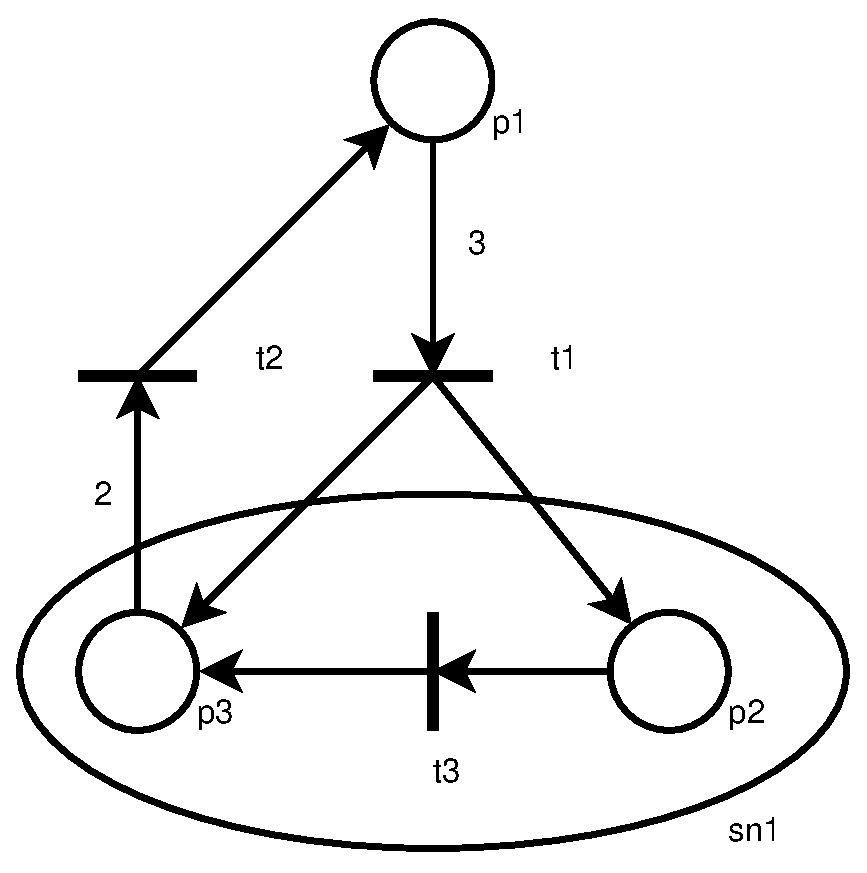
\includegraphics[width=0.4\textwidth]{figures/PNML-RdPSubred.eps}\end{matrix}
\pause \Rightarrow 
 \begin{matrix} 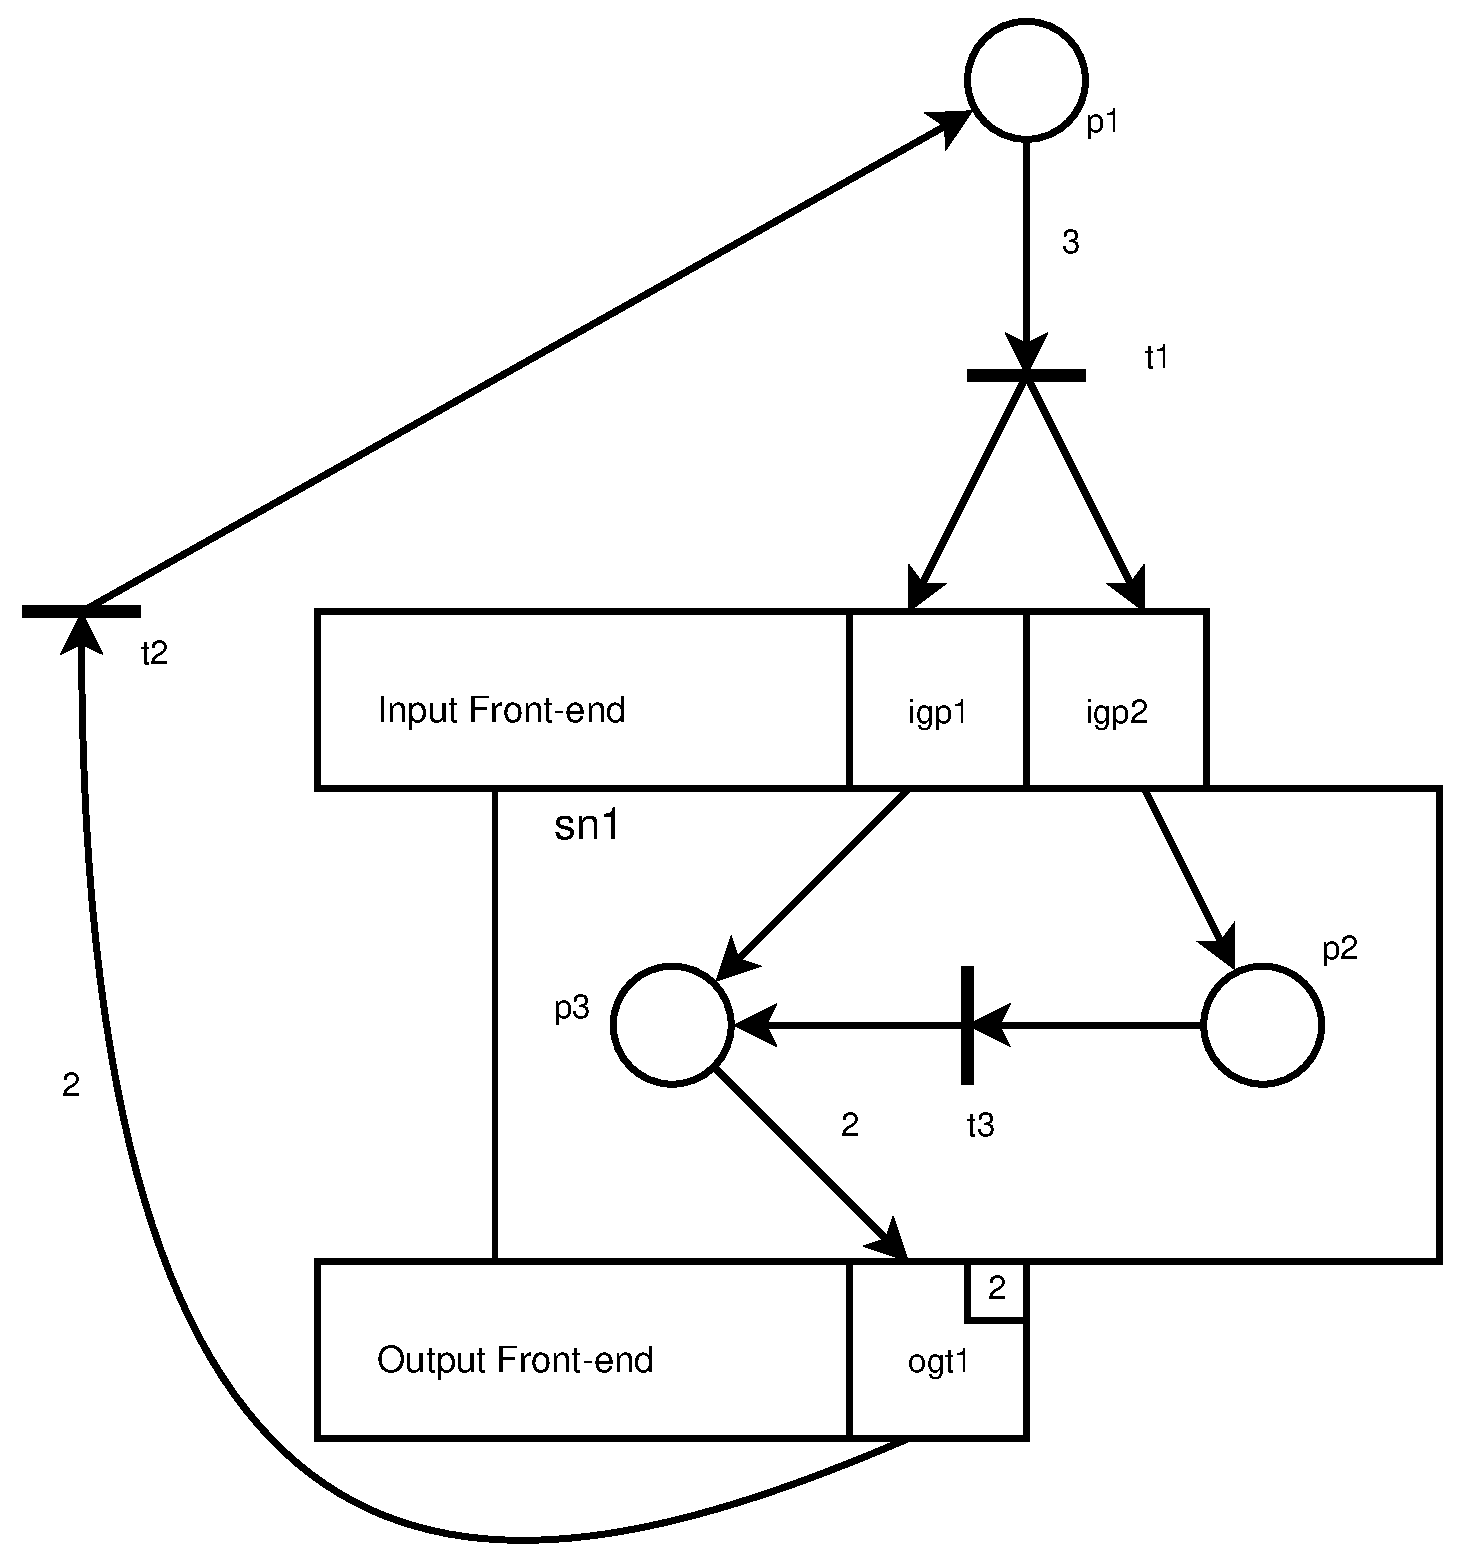
\includegraphics[width=0.58\textwidth]{figures/PNML-SubredEjemplo1.eps}\end{matrix}
\]
\end{slide}







\begin{slide}[toc=Extensi\'on PNML V, method=file]{Ejemplo extensi\'on PNML}
\begin{multicols}{2}
\begin{lstlisting}[basicstyle=\ttfamily\tiny]
<subnet id="sn1">
  <interface id="sn1-interface">
    <gate id="igp1" action="input" type="place"/>
    <gate id="igp2" action="input" type="place"/>
    <gate id="ogt1" action="output" type="transition">
      <inscription>
        <text> 2 </text>
      </inscription>
    </gate>
  </interface>
  <content id="sn1-content">
    <place id="p2"/>
    <place id="p3"/>
    <transition id="t3"/>
    <arc id="sn1-a2" source="igp2" target="p2"/>
    <arc id="sn1-a3" source="igp1" target="p3"/>
    <arc id="sn1-a4" source="p3" target="ogt1">
      <inscription>
        <text> 2 </text>
      </inscription>
    </arc>
    <arc id="a5" source="t3" target="p3"/>
    <arc id="a6" source="p2" target="t3"/>
  </content>
</subnet>
<place id="p1"/>
<transition id="t1"/>
<transition id="t2"/>
<arc id="a1" source="p1" target="t1">
  <inscription>
    <text> 3 </text>
  </inscription>
</arc>
<arc id="a2" source="t1" target="igp2"/>
<arc id="a3" source="t1" target="igp1"/>
<arc id="a4" source="ogt1" target="t2">
  <inscription>
    <text> 2 </text>
  </inscription>
</arc>
<arc id="a7" source="t2" target="p1"/>
\end{lstlisting}
\end{multicols}
\end{slide}







\section{Seguridad en redes de Petri}
\begin{slide}{Seguridad}

\begin{itemize}
\item \textbf{Privacidad}. Determinadas partes de la red deben ser ocultadas:
el contenido es secreto, por lo que no todo el mundo deber\'ia poder conocerlo.
\pause
\item \textbf{Integridad}. Cualquier cambio en las partes securizadas
debe ser detectado. Si cualquiera de estas partes sufre cualquier tipo de
modificaci\'on, la informaci\'on puede haberse visto comprometida y quiz\'a no
sea v\'alida o correcta. Pero no podemos saber lo que se ha cambiado: s\'olo
podemos detectar que el original ha sido alterado.
\pause
\item \textbf{Autenticaci\'on}. Puedo autenticar el origen de la red/subred
(firmador, autor o validador).
\pause
\item \textbf{No repudio}. Con esta caracter\'istica, se evita la posibilidad de suplantar a otra persona es evitada. Por tanto, aquel que firma una parte
no puede decir que no lo ha hecho: el firmante no puede negar que lo es.
\end{itemize}

\end{slide}





\begin{slide}{Selecci\'on de subredes: XPath}
Podemos aplicar seguridad a:
\begin{itemize}
\item La red de Petri entera
\item S\'olo a determinadas partes de ella
\end{itemize}
\pause
\bigskip
La manera est\'andar es el uso de expresiones XPath, que devuelve el conjunto
de nodos xml que tienen que ser procesados (cifrados o firmados).
Por ejemplo:
\begin{itemize}
\item '\texttt{/}' - Indica la red completa, el nodo ra\'iz
\item '\texttt{/pnml/net/page/subnet[@id="sn1"]}' - Indica que s\'olo debe
procesarse la subred con id="sn1"
\item '\texttt{/pnml/net/page/subnet}' - Indica que deben procesarse todas
las subredes
\end{itemize}
\end{slide}




\begin{slide}[toc=XMLEncryption, method=file]{XMLEncryption}
XMLEncryption asegura la privacidad:
\begin{lstlisting}
  <content id="sn1-content">
    <place id="p2"/>
    <place id="p3"/>
    <transition id="t3"/>
    <arc id="sn1-a2" source="igp2" target="p2"/>
    <arc id="sn1-a3" source="igp1" target="p3"/>
    <arc id="sn1-a4" source="p3" target="ogt1">
      <inscription>
        <text> 2 </text>
      </inscription>
    </arc>
    <arc id="a5" source="t3" target="p3"/>
    <arc id="a6" source="p2" target="t3"/>
  </content>
\end{lstlisting}
\end{slide}





\begin{slide}[toc=XMLEncryption II, method=file]{XMLEncryption}
\begin{lstlisting}
<content id="sn1-content">
 <xenc:EncryptedData xmlns:xenc="http://www.w3.org/2001/04/xmlenc#"  
    Type="http://www.w3.org/2001/04/xmlenc#Element">  
  <xenc:EncryptionMethod  
      Algorithm="http://www.w3.org/2001/04/xmlenc#aes128-cbc"  
      xmlns:xenc="http://www.w3.org/2001/04/xmlenc#" />  
  <xenc:CipherData  
      xmlns:xenc="http://www.w3.org/2001/04/xmlenc#">  
   <xenc:CipherValue  
       xmlns:xenc="http://www.w3.org/2001/04/xmlenc#">  
         Wr1njyJlYYOM9lAYqcwGCWkw2L4pUjQD2GGVoU9lVZ0wKqHY8y3lGY8FY4i5K
         AGY8FY4i5K3G8grIe1HRFqe7RtkFiXZgGMeYnQp6oB6ckKp3KFKHVqtucc9rA
         VzOgC7XAwe61HRFqe6RRVzXjNM9hlVZ0wKqHY8y3l3GY8FY4i5K3G8grIe2xN
         xfw17hoYCUdwkzM12iiBJaKQcZcAALcLX2RTF9McAJOElonRrNdUgi9SCBz5Z
         kPdQCFJaGFAoKYmDZF9OjTBQ4qf9FVf8OsUXSxqRnXUeUZEB7rhgVY68gyCp4
         TGPZOWz/Yb7Sbq1pNiG6wqNbsepKWG9EV6n9rjSfiOocvy9wL8m1I0HmAp2l4
         RRVzXjNMLU5ZgGMeYny8NVPQmUSDX7NRtnR6YnQp6oB6GY8F=
   </xenc:CipherValue>  
  </xenc:CipherData>  
 </xenc:EncryptedData>
</content>
\end{lstlisting}
\end{slide}




\begin{slide}[toc=XMLEncryption III]{XMLEncryption}
\begin{multicols}{2}
Se permite la sustituci\'on de una red cifrada por otra:
\begin{itemize}
\item Quitar la subred a eliminar del c\'odigo fuente xml
\item Insertar la nueva red cifrada en el c\'odigo xml
\item Modificar los id de los arcos que entran o salan para hacerlos coincidir
con el nuevo nombre de las puertas
\end{itemize}
\[
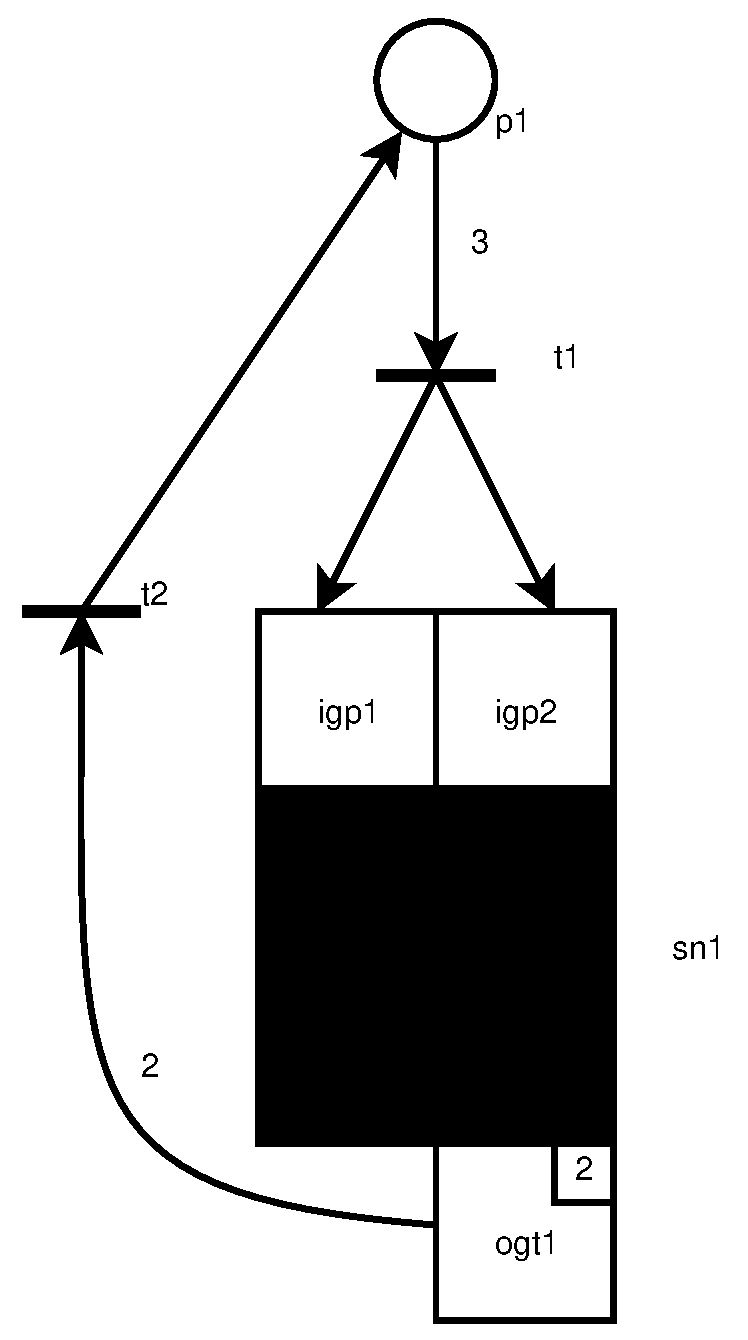
\includegraphics[width=0.36\textwidth]{figures/XMLENC-SubredEjemplo1.eps}
\]
\end{multicols}
\end{slide}






\begin{slide}[toc=XMLSignature]{XMLSignature}
\begin{itemize}
\item \begin{large}XMLSignature provee los servicios de \textbf{integridad,
autenticaci\'on y no repudio}.
\end{large}
\pause\bigskip
\item \begin{large}La firma digital se anexa en el documento con datos para
la correcta verificaci\'on de la misma
\end{large}
\end{itemize}
\end{slide}




\begin{slide}[method=file, toc=XMLSignature II]{XMLSignature}
\begin{lstlisting}[basicstyle=\ttfamily\tiny]
  <ds:Signature xmlns:ds="http://www.w3.org/2000/09/xmldsig#">
    <ds:SignedInfo>
      <ds:CanonicalizationMethod Algorithm="http://www.w3.org/TR/2001/REC-xml-c14n-20010315"/>
      <ds:SignatureMethod Algorithm="http://www.w3.org/2000/09/xmldsig#rsa-sha1"/>
      <ds:Reference URI="">
        <ds:Transforms>
          <ds:Transform Algorithm="http://www.w3.org/2000/09/xmldsig#enveloped-signature"/>
          <ds:Transform Algorithm="http://www.w3.org/TR/2001/REC-xml-c14n-20010315#WithComments"/>
          <ds:Transform Algorithm="http://www.w3.org/2002/06/xmldsig-filter2">
            <dsig-xpath:XPath xmlns:dsig-xpath="http://www.w3.org/2002/06/xmldsig-filter2" Filter="intersect">
              /pnml/net/page/subnet[@id="sn1"]
            </dsig-xpath:XPath>
          </ds:Transform>
        </ds:Transforms>
        <ds:DigestMethod Algorithm="http://www.w3.org/2000/09/xmldsig#sha1"/>
        <ds:DigestValue>prCzhLgTCZ1ck6MjQnFy6cASCZw=</ds:DigestValue>
      </ds:Reference>
    </ds:SignedInfo>
    <ds:SignatureValue>
      QoO7mQmGBFTg2UxgiZnzlsnKi8V477JC0v12JPItL53zIOCpjhOwLoyxENl6v8lCLoJ9WwFHlBKk
      r3GdqrgZimNXMUjwR4zkd9FVNcIrn85DuRjHAazDwSuPMq9w0N5A07c0xJ24uvn9zzpbQxfblYTb
      kiy08+S0pqczUfbv52g=
    </ds:SignatureValue>
    
    ...........
\end{lstlisting}
\end{slide}



\begin{slide}[method=file, toc=XMLSignature III]{XMLSignature}
\begin{lstlisting}[basicstyle=\ttfamily\tiny]
    ...........
    <ds:KeyInfo>
      <ds:X509Data>
        <ds:X509Certificate>
          MIICgTCCAeqgAwIBAgIETfh4CTANBgkqhkiG9w0BAQUFADCBhDELMAkGA1UEBhMCRVMxETAPBgNV
          BAgTCExBIFJJT0pBMREwDwYDVQQHDAhMT0dST8KlTzEgMB4GA1UEChMXVU5JVkVSU0lEQUQgREUg
          TEEgUklPSkExDDAKBgNVBAsTA1BGQzEfMB0GA1UEAwwWScKlSUdPIExFw6BOIFNBTUFOSUVHTzAe
          Fw0xMTA2MTUwOTE0NDlaFw0xMTA5MTMwOTE0NDlaMIGEMQswCQYDVQQGEwJFUzERMA8GA1UECBMI
          TEEgUklPSkExETAPBgNVBAcMCExPR1JPwqVPMSAwHgYDVQQKExdVTklWRVJTSURBRCBERSBMQSBS
          SU9KQTEMMAoGA1UECxMDUEZDMR8wHQYDVQQDDBZJwqVJR08gTEXDoE4gU0FNQU5JRUdPMIGfMA0G
          CSqGSIb3DQEBAQUAA4GNADCBiQKBgQChePFNVCIfphFlyXQ9BysiR5BfXIuv3AnAK80Fuw4tTFwC
          nVUjJeGnkUYQO32oUuffEBK8WsEqjeH8A7zrHTRQjfYZWyuGWrM8gJXOa5P0MROPm7c3H8b5a6Nx
          Fc2zLwR0tYkqLI2xqDOFII2RwK5L2yGeV4T4y8i3h1U0OFTSEwIDAQABMA0GCSqGSIb3DQEBBQUA
          A4GBAIDOvAAdOCaTpya83bGB2KmngMJrNxxWDpAi5LGFrN8iCShmbTpIeIbYBUAaBpZtdhOnhq4n
          wD5QOENSFipQcdH5GEpPM9Rquy6xMwfda9EU5UfOSEmbk4fK2vaIOVjynpQsJ9P99enO2smQlyvw
          DhBa7Xacz6qDut8ghUeuV5Js
        </ds:X509Certificate>
      </ds:X509Data>
      <ds:KeyValue>
        <ds:RSAKeyValue>
          <ds:Modulus>
            oXjxTVQiH6YRZcl0PQcrIkeQX1yLr9wJwCvNBbsOLUxcAp1VIyXhp5FGEDt9qFLvnxASvFrBKo3h
            sAO86x00UI32GVsrhlqzPICVzmvz9DETj5v3Px4GdWujcdfasy8EdLWJKiyNsagzhSCNkcCuS9sh
            nleE8MvIt4dVNDhU0hM=
          </ds:Modulus>
          <ds:Exponent>AQAB</ds:Exponent>
        </ds:RSAKeyValue>
      </ds:KeyValue>
    </ds:KeyInfo>
  </ds:Signature>
\end{lstlisting}
\end{slide}





\begin{slide}{Seguridad integral}
Aspectos a tener en cuenta
\begin{itemize}
\item XMLEncryption \textbf{sustitu\'ia} el contenido
en claro por el contenido cifrado. Sin embargo, XMLSignature \textbf{adjunta} informaci\'on
adicional con datos de la firma. Esto permite tener varias firmas sobre el
mismo contenido.
\pause\bigskip
\item En XMLEncryption se pu�ede sustituir una subred por otra con el mismo
front-end. Sin embargo, esto no es posible si la subred est\'a firmada con
XMLSignature ya que detectar\'ia cambios
\pause\bigskip\item En el caso de subredes firmadas y cifradas, el orden en el que se aplican
estas t\'ecnicas es importante y depende de lo que quiera el gestor.
\end{itemize}
\end{slide}






\section{Conclusiones}
\begin{slide}{Conclusiones}
He desarrollado un m\'etodo exhaustivo para definir subredes con interfaces.
La interacci\'on entre estas subredes y el resto de la red se realiza siempre
a trav\'es de sus front-ends. El m\'etodo de representaci\'on elegido ha sido
PNML. Una vez realizado esto, la conclusi\'on de este trabajo es mostrar que
es posible aplicar medidas de seguridad a redes de Petri para ampliar en
4 caracter\'isticas adicionales a estas redes (o subredes):
\begin{itemize}
\item Privacidad: no todos pueden acceder a algunos datos
\item Integridad: se detectan cambios no permitidos
\item Autenticacion: asegura la autor\'ia de alguna informaci\'on
\item No repudio: una persona no puede suplantar a otra
\end{itemize}
Con XMLEncryption conseguimos privacidad. Integridad, autenticaci\'on y no
repudio se obtienen con XMLSignature
\end{slide}






\begin{slide}{Publicaciones}
\textbf{Art\'iculos en Congresos Internacionales}
\begin{scriptsize}
\begin{itemize}
\item EMSS Roma 2011. Security and Protection in Petri Nets sending and storage. Signing and Encryption.
\item EMSS Atenas 2013. Analysis of information partial encryption options for exchanging Petri Nets systems
\item EMSS Burdeos 2014. Petri net representation with ciphered subnets: definition of PNML extensions for subnets representation and use of XMLEncryption for ciphering.
\item EMSS Bergeggi 2015.  Validation and approval of Petri Net ciphered subnets: security in Petri Nets sharing and storage using PNML, XMLSecurity and XMLSignature
\end{itemize}
\end{scriptsize}
\textbf{Premios}
\begin{scriptsize}
\begin{itemize}
\item Premio al mejor estudiante de doctorado en el EMSS Burdeos 2014\end{itemize}
\end{scriptsize}
\textbf{Art\'iculos enviados a revistas}
\begin{scriptsize}
\begin{itemize}
\item Journal of Computation Science. Security and Protection in Petri Nets sending and storage. Signing and Encryption
\item Simulation, modelling practice and theory.
Validation and approval of Petri Net ciphered subnets: security in Petri Nets sharing and storage using PNML, XMLSecurity and XMLSignature\end{itemize}
\end{scriptsize}
\end{slide}


\begin{slide}{Gracias}

\bigskip
\bigskip
\bigskip
\bigskip
\bigskip
\bigskip
\begin{center}
\huge{Gracias por su atenci\'on}
\end{center}
\end{slide}





\end{document}


